\documentclass{beamer}
\usepackage[utf8]{inputenc}
\usepackage[spanish]{babel}
\usepackage{graphicx,hyperref,ru,url}

% The title of the presentation:
%  - first a short version which is visible at the bottom of each slide;
%  - second the full title shown on the title slide;
\title[Mathematical model of Guinea Worm Disease]{
  A mathematical model for the eradication of Guinea Worm Disease}

% Optional: a subtitle to be dispalyed on the title slide
\subtitle{Robert J. Smith, Patrick Cloutier, James Harriso and Alex Desforges}

% The author(s) of the presentation:
%  - again first a short version to be displayed at the bottom;
%  - next the full list of authors, which may include contact information;
\author[Bartolomé Ortiz Viso]{
  Bartolomé Ortiz Viso \\\medskip
  {\small \url{bortiz@correo.ugr.es}} \\ 
  {\small \url{@bortizmath}}}

% The institute:
%  - to start the name of the university as displayed on the top of each slide
%    this can be adjusted such that you can also create a Dutch version
%  - next the institute information as displayed on the title slide
\institute[Universidad de Granada]{
  Modelos en Ecología  \\
  Máster en Física y Matemáticas}

% Add a date and possibly the name of the event to the slides
%  - again first a short version to be shown at the bottom of each slide
%  - second the full date and event name for the title slide
\date[2 Febrero, 2018]{2 Febrero, 2018}

\begin{document}

\begin{frame}
  \titlepage
\end{frame}

\begin{frame}
  \frametitle{Índice}

  \tableofcontents
\end{frame}

\section{Introducción}

\begin{frame}
  \frametitle{Introducción}
		\begin{block}{Claves de la Dracunculiasis}
			\begin{itemize}
				\item Los europeos vieron por primera vez la enfermedad en la costa de Guinea del oeste de África en
				el siglo XVII .
				\item  En la década de 1950 había 50 millones de casos.
				\item  En 1986 comenzó un programa de erradicación concertado.
				\item  Si se erradica con éxito, será el primer parásito
				enfermedad a ser erradicada.
				\item  GWD es la única enfermedad que se transmite únicamente a través del agua potable.
			\end{itemize}
		\end{block}
\end{frame}

\section{Mecanismos biológicos implicados}

\begin{frame}
  \frametitle{Mecanismos biológicos implicados}
	\begin{figure}
		\centering
		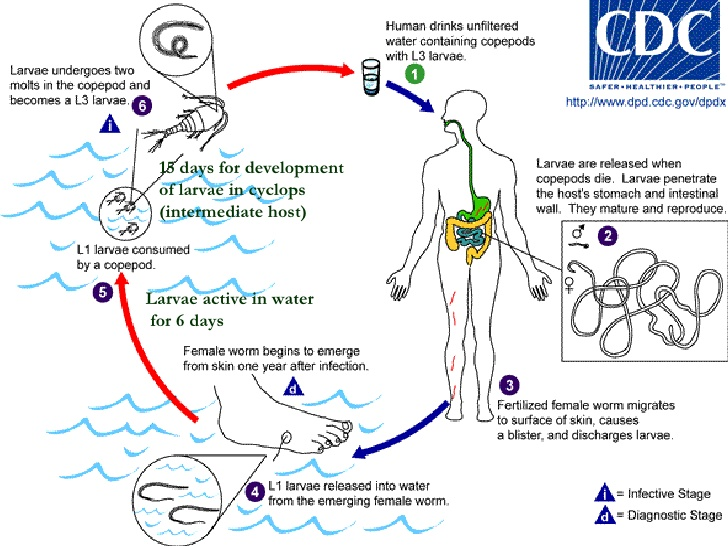
\includegraphics[width=0.7\textwidth]{diagrama.jpg}
		\caption{Ciclo de la dracunculiasis }
		\label{fig:1}
	\end{figure}
\end{frame}



\section{Modelado matemático}


\begin{frame}
  \frametitle{Modelo final}
  \begin{block}{Variables}
  	S: Susceptibles, E: Expuestos, I: Infectados, W: Cantidad de parásito
  \end{block}
  \begin{equation}
  S'=\Pi-\beta SW-\mu S+\kappa I, \text{ para }t\neq t_k
  \end{equation}
  \begin{equation}
  E'=\beta S W -\alpha E -\mu E, \text{ para }t\neq t_k
  \end{equation}
  \begin{equation}
  I'=\alpha E-\kappa I -\mu I, \text{ para }t\neq t_k
  \end{equation}
  \begin{equation}
  W'=\gamma I - \mu_W W,  \text{ para }t\neq t_k
  \end{equation}
  \begin{equation}
  \Delta W= -rW   \text{ para }t=t_k
  \end{equation}
\end{frame}




\subsection{Comportamiento sin impulsos}

\begin{frame}
	\frametitle{Comportamiento sin impulsos}
    \begin{block}{Resultados teóricos}
	  \begin{itemize}
		\item Dos posibles comportamientos dependientes de $R_0$
		\item $R_0= \frac{\Pi \alpha\gamma\beta}{\mu(\alpha+\mu)(\kappa+\mu)\mu_W}$
		\item Si $R_0<1$ el unico punto de equilibrio es $(A,E,I,W)=(\frac{\Pi}{\mu},0,0,0)$ y es estable
		\item Si $R_0>1$ el equilibrio libre de enfermedad es inestable  y existe un equilibrio estable con enfermedad
	  \end{itemize}	
	\end{block}
\end{frame}

\subsection{Comportamiento con impulsos}
\begin{frame}
	\frametitle{Comportamiento con impulsos}
	\begin{block}{Planteamiento}
		El sistema con impulsos se puede analizar sobreestimando cantidades. Esto nos permite resolver la ecuacion para W.
	\end{block}
	\begin{columns}[t]
		
		\column{0.5\textwidth}
		\begin{block}{Impulsos periodicos}
		\begin{itemize}
			\item Disminucion gradual empezando por el equilibrio
		\end{itemize}
	\end{block}
		\column{0.5\textwidth}
		\begin{block}{Impulsos NO periodicos}
		\begin{itemize}
			\item Disminucion gradual empezando por el equilibrio, si la estimacion del espaciado es correcta
		\end{itemize}
	\end{block}
	\end{columns}
	
\end{frame}


\section{Simulaciones numéricas}
\begin{frame}
	\frametitle{Simulaciones numéricas}
	\begin{block}{Objetivo}
Calcular la sensibilidad de el estimador $R_0$
	\end{block}
	\begin{itemize}
		\item Latin hypercube sampling (LHS)
		\item Partial rank correlation
		coefficients (PRCCs)
	\end{itemize}
	\begin{figure}[resultados]
		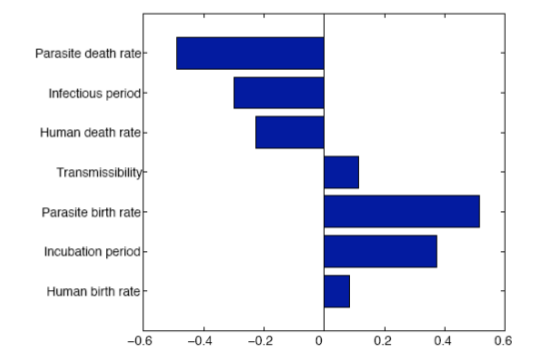
\includegraphics[scale=0.4]{rangos.png}
		\label{rangos}
	\end{figure}
\end{frame}


\subsection{Simulación caso particular}
\begin{frame}
		\frametitle{Simulación caso particular}
		Nos llevamos el problema a un esquema discreto
\end{frame}

\section{Conclusiones y futuro trabajo}

\begin{frame}
	\frametitle{Conclusiones y futuro trabajo}


\begin{itemize}
	\item La clorizacion no ocurre de forma simultanea
	\item Hay distintas fuentes de agua a considerar y por ende distintos focos
	\item El ciclo de vida no se ve reflejado en el modelo.
	\item Necesaria la interpretación matemática incluso para variables no biológicas.
\end{itemize}
\end{frame}
\end{document}